% This is samplepaper.tex, a sample chapter demonstrating the
% LLNCS macro package for Springer Computer Science proceedings;
% Version 2.21 of 2022/01/12
%
\documentclass[runningheads]{llncs}
%
\usepackage[T1]{fontenc}
% T1 fonts will be used to generate the final print and online PDFs,
% so please use T1 fonts in your manuscript whenever possible.
% Other font encondings may result in incorrect characters.
%
\usepackage{graphicx}
\usepackage{hyperref}
% Used for displaying a sample figure. If possible, figure files should
% be included in EPS format.
%
% If you use the hyperref package, please uncomment the following two lines
% to display URLs in blue roman font according to Springer's eBook style:
\usepackage{color}
\renewcommand\UrlFont{\color{blue}\rmfamily}
\urlstyle{rm}

\usepackage{amsmath}
\usepackage{amssymb}
\usepackage{tikz}
\usepackage{wrapfig}
\usepackage{environ}

\usepackage{changes}
\usepackage{algorithm}
\usepackage{algpseudocode}
\usepackage{varwidth}
\usepackage{mathtools}
\setauthormarkup{}
\definechangesauthor[name=jo, color=magenta]{JO}
\definechangesauthor[name=rom, color=teal]{ROM}

% set of real numbers
\newcommand{\R}{\ensuremath{\mathbb{R}}}
% set of integer numbers
\newcommand{\Z}{\ensuremath{\mathbb{Z}}}
% cell complex build on the lattice \Z^d
\let\C\relax \DeclareMathOperator{\C}{\ensuremath{\mathcal{C}^d}} % modified because of incompatiblity with hyperref package
% cardinality of a set
\newcommand{\Card}[1]{\ensuremath{\#\left( #1 \right)}}
% Interior of a closed set.
\newcommand{\Int}[1]{\ensuremath{\mathrm{Int}\left( #1 \right)}}
% Some vectors and matrices
\newcommand{\vx}[0]{\ensuremath{\mathbf{x}}}
\newcommand{\vy}[0]{\ensuremath{\mathbf{y}}}
\newcommand{\vz}[0]{\ensuremath{\mathbf{z}}}
\newcommand{\vb}[0]{\ensuremath{\mathbf{b}}}
\newcommand{\vA}[0]{\ensuremath{\mathbf{A}}}
\newcommand{\va}[0]{\ensuremath{\mathbf{a}}}
\newcommand{\vc}[0]{\ensuremath{\mathbf{c}}}
\newcommand{\ve}[0]{\ensuremath{\mathbf{e}}}
\newcommand{\vm}[0]{\ensuremath{\mathbf{m}}}
\newcommand{\vn}[0]{\ensuremath{\mathbf{n}}}
\newcommand{\vu}[0]{\ensuremath{\mathbf{u}}}
\newcommand{\vv}[0]{\ensuremath{\mathbf{v}}}
\newcommand{\vw}[0]{\ensuremath{\mathbf{w}}}
\newcommand{\vp}[0]{\ensuremath{\mathbf{p}}}
\newcommand{\vq}[0]{\ensuremath{\mathbf{q}}}
\newcommand{\vr}[0]{\ensuremath{\mathbf{r}}}
\newcommand{\vs}[0]{\ensuremath{\mathbf{s}}}
\newcommand{\vt}[0]{\ensuremath{\mathbf{t}}}
% Convex hull
\newcommand{\Conv}[1]{\mathrm{CvxH}\left( #1 \right)}

% References
\newcommand{\Equ}[1]{(\ref{#1})}
\newcommand{\RefFigure}[1]{Figure~\ref{#1}}
\newcommand{\RefLemma}[1]{Lemma~\ref{#1}}
\newcommand{\RefLemmas}[2]{Lemmas~\ref{#1} and~\ref{#2}}
\newcommand{\RefTheorem}[1]{Theorem~\ref{#1}}
\newcommand{\RefCorollary}[1]{Corollary~\ref{#1}}
\newcommand{\RefAlgorithm}[1]{Algorithm~\ref{#1}}
\newcommand{\RefSection}[1]{Section~\ref{#1}}
\newcommand{\Refline}[1]{line~\ref{#1}}
\newcommand{\RefLine}[1]{Line~\ref{#1}}

% Star, closure, boundary of a complex
\newcommand{\Bd}[1]{\ensuremath{\mathrm{Bd}\left(#1\right)}}
\newcommand{\Star}[1]{\ensuremath{\mathrm{Star}\left(#1\right)}}
\newcommand{\Starop}[0]{\ensuremath{\mathrm{Star}}}
\newcommand{\Cl}[1]{\ensuremath{\mathrm{Cl}\left(#1\right)}}
% Closed interior
\newcommand{\CI}[1]{\ensuremath{\mathrm{ClInt}\left(#1\right)}}
% Body of a complex
\newcommand{\Body}[1]{\ensuremath{\left\|#1\right\|}}
% topological closure
\newcommand{\TCl}[1]{\ensuremath{\overline{#1}}}
% topological interior
\newcommand{\TInt}[1]{\ensuremath{\mathring{#1}}}
% topological boundary
\newcommand{\TBd}[1]{\ensuremath{\partial{#1}}}
% <=
\newcommand{\Le}{\ensuremath{\leqslant}}
% >=
\newcommand{\Ge}{\ensuremath{\geqslant}}


% Euclidean distance
\newcommand{\EDist}[0]{\ensuremath{\mathrm{d}_\mathbf{E}}}
% Hausdorff distance
\newcommand{\HDist}[0]{\ensuremath{\mathrm{d}_H}}
% Normal cone to S at p
\newcommand{\NC}[2]{\ensuremath{\mathrm{N}_{#1}(#2)}}

% l2 norm
\newcommand{\ltwo}[0]{\ensuremath{\ell_2}}
\newcommand{\loo}[0]{\ensuremath{\ell_\infty}}

% Reach
\newcommand{\Reach}[1]{\ensuremath{\mathrm{reach}(#1)}}
% Volume
\newcommand{\Vol}[1]{\ensuremath{\mathrm{Vol}\left(#1\right)}}
\newcommand{\Vold}[2]{\ensuremath{\mathrm{Vol}^{#1}\left(#2\right)}}
% Digitization
\newcommand{\Dig}[2]{\ensuremath{\mathrm{D}_{#1}\left(#2\right)}}
% Counting lattice points
\newcommand{\Lat}[1]{\ensuremath{\mathcal{L}_{#1}}}
\newcommand{\LatC}[2]{\ensuremath{\Lat{#1}(#2)}}


%
\begin{document}
%
    \title{Fast and exact visibility on digitized shapes and application to feature-aware normal estimation}
%
    \titlerunning{Fast and exact visibility on digitized shapes}
% If the paper title is too long for the running head, you can set
% an abbreviated paper title here
%
    \author{Romain Negro\inst{1}\orcidID{0000-XXXX-YYYY-ZZZZ} \and
    Jacques-Olivier Lachaud\inst{1}\orcidID{0000-0003-4236-2133}}
%
    \authorrunning{R. Negro and J.-O. Lachaud}
% First names are abbreviated in the running head.
% If there are more than two authors, 'et al.' is used.
%
    \institute{Universit\'e Savoie Mont Blanc, CNRS, LAMA, F-73000 Chambéry, France\\
    \email{\{romain.negro|jacques-olivier.lachaud\}@univ-smb.fr}}
%
    \maketitle              % typeset the header of the contribution
%
    \begin{abstract}
        Our abstract
        \keywords{Visibility \and Geometric inference \and Digital normal estimation \and Digital geometry}
    \end{abstract}

%%%%%%%%%%%%%%%%%%%%%%%%%%%%%%%%%%%%%%%%%%%%%%%%%%%%%%%%%%%%%%%%%%%%%%


    \section{Introduction}


    Visibility is a fundamental concept in computational geometry and digital topology, with applications ranging from computer vision to geometric modeling.
    In this work, we explore visibility through the lens of chord tangency, introducing a novel approach that builds on discrete geometric structures.
    Our framework leverages the discrete setting of and cell complexes, providing a rigorous foundation for analyzing visibility properties in digital spaces.

    We recall essential definitions from previous works, particularly the notions of cell complexes and the star operator as formalized in~\cite{lachaud:2021-dgmm} and~\cite{lachaud:2022-jmiv}.
    The integer grid serves as our primary space of study, where geometric structures are discretized using cell complexes.
    A cell complex is a decomposition of space into elementary units (vertices, edges, faces, and higher-dimensional counterparts) forming a combinatorial representation of geometric objects.
    The star of a cell, as defined in these works, consists of all higher-dimensional cells that contain it, a crucial concept for analyzing local neighborhoods and connectivity.

    Building on these foundations, our study focuses on visibility as determined by the tangency of chords in discrete geometry.
    We define and analyze how visibility relationships emerge in this context and investigate their combinatorial and topological implications.
    This approach provides a new perspective on discrete visibility, offering potential applications in digital imaging, surface reconstruction, and computational topology.

    The remainder of this paper is structured as follows.
    In Section 2, we formalize the concept of chord tangency and its role in visibility analysis.
    Section 3 enters into the usage of integer intervals intersections to quickly scan the figure in order to recover this visibiltiy.
    Section 4 presents our main results, using this visibility to compute normals using the CNC estimator~\cite{lachaud:2022-dcg}.
    Finally, Section 5 concludes with some other applications of integer intervals intersections in the field.


%%%%%%%%%%%%%%%%%%%%%%%%%%%%%%%%%%%%%%%%%%%%%%%%%%%%%%%%%%%%%%%%%%%%%%


    \section{Visibility through tangency of chords}


    Let $\Z^d$ be the d-dimensional digital space, $d$ > 0.
    Let $\mathcal{C}^d$ be the (cubical) cell complex induced by the lattice $\Z^d$ : its 0-cells are the points of $\Z^d$, its 1-cells are the open unit segments joining two 0-cells at distance 1, its 2-cells are the open unit squares, etc., and its d-cells are the d-dimensional open unit hypercubes with vertices in $\Z^d$.
    We denote $\mathcal{C}^d_k$ the set of its k-cells.
    In the following, a cell will always designate an element of $\mathcal{C}^d$, and the term subcomplex always designates a subset of $\mathcal{C}^d$.

    A cell $\sigma$ is a face of another cell $\tau$ whenever $\sigma$ is a subset of the topological closure $\bar{\tau}$ of $\tau$, written $\sigma \preccurlyeq \tau$.
    Given any subcomplex K of $\mathcal{C}^d$, the star $Star(K)$ of K is $\{\tau \in \mathcal{C}^d, s.t.\ \exists\sigma \in K,\sigma \preccurlyeq \tau\}$

    \begin{definition}
        Two points \( p \) and \( q \) on \( K \) are visible if and only if the segment \([p, q]\) is included in \(\text{Star}(K)\), i.e., \( [p, q] \subseteq \text{Star}(K)\)
    \end{definition}

    % Examples of visibility in 2D
    \begin{figure}
        \centering
        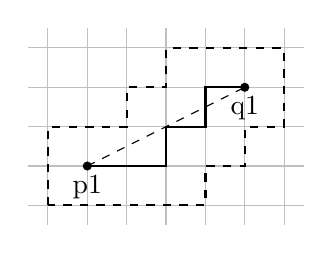
\begin{tikzpicture}
            \draw[step=0.5,lightgray,thin,xshift=-1cm,yshift=-1cm] (0.25,0.25) grid (3.75,2.75);
            \draw[dashed] (0,0) -- (2,1);
            \filldraw[black] (0,0) circle (0.05) node[anchor=north] {p1};
            \filldraw[black] (2,1) circle (0.05) node[anchor=north] {q1};
            \draw [thick] (0,0) -- (0.5,0) -- (1,0) -- (1,0.5) -- (1.5,0.5) -- (1.5,1) -- (2,1);
            \draw[thick,dashed] (-0.5,-0.5) -- (-0.5,0.5) -- (0.5,0.5) -- (0.5,1) -- (1,1) -- (1,1.5) -- (2.5,1.5) -- (2.5,0.5) -- (2,0.5) -- (2,0) -- (1.5,0) -- (1.5,-0.5) -- (-0.5,-0.5);
        \end{tikzpicture}
        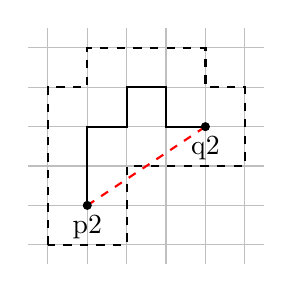
\begin{tikzpicture}
            \draw[step=0.5,lightgray,thin,xshift=-1cm,yshift=-1cm] (0.25,0.25) grid (3.25,3.25);
            \draw[red,dashed,thick] (0,0) -- (1.5,1);
            \filldraw[black] (0,0) circle (0.05) node[anchor=north] {p2};
            \filldraw[black] (1.5,1) circle (0.05) node[anchor=north] {q2};
            \draw [thick] (0,0) -- (0,1) -- (0.5,1) -- (0.5,1.5) -- (1,1.5) -- (1,1) -- (1.5,1);
            \draw[thick,dashed] (-0.5,-0.5) -- (-0.5,1.5) -- (0,1.5) -- (0,2) -- (1.5,2) -- (1.5,1.5) -- (2,1.5)  -- (2,0.5) -- (0.5,0.5) -- (0.5,-0.5) -- (-0.5,-0.5);
        \end{tikzpicture}
        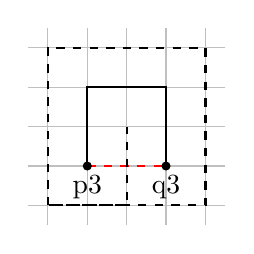
\begin{tikzpicture}
            \draw[step=0.5,lightgray,thin,xshift=-1cm,yshift=-1cm] (0.25,0.25) grid (2.75,2.75);
            \draw[red,dashed,thick] (0,0) -- (1,0);
            \filldraw[black] (0,0) circle (0.05) node[anchor=north] {p3};
            \filldraw[black] (1,0) circle (0.05) node[anchor=north] {q3};
            \draw [thick] (0,0) -- (0,1) -- (1,1) -- (1,0);
            \draw[thick,dashed] (-0.5,-0.5) -- (-0.5,1.5) -- (1.5,1.5) -- (1.5,-0.5) -- (-0.5,-0.5) -- (0.5,-0.5) -- (0.5,0.5);
        \end{tikzpicture}
        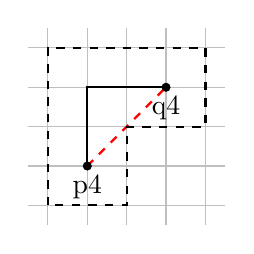
\begin{tikzpicture}
            \draw[step=0.5,lightgray,thin,xshift=-1cm,yshift=-1cm] (0.25,0.25) grid (2.75,2.75);
            \draw[red,dashed,thick] (0,0) -- (1,1);
            \filldraw[black] (0,0) circle (0.05) node[anchor=north] {p4};
            \filldraw[black] (1,1) circle (0.05) node[anchor=north] {q4};
            \draw [thick] (0,0) -- (0,1) -- (1,1);
            \draw[thick,dashed] (-0.5,-0.5) -- (-0.5,1.5) -- (1.5,1.5) -- (1.5,0.5) -- (0.5,0.5) -- (0.5,-0.5) -- (-0.5,-0.5);
        \end{tikzpicture}
        \caption{Examples of visibility in 2D, only q1 is visible from p1, q2 is not visible from p2 (gets out of the star), q3 is not visible from p3 (gets out of the star from a 1-d cell), q4 is not visible from p4 (gets out of the star from a 0-d cell).}
        \label{fig:visibility-2d}
    \end{figure}


    We note that one particular aspect of this visibility definition is that all visible points from a given point taken as a separate complex are not necessarily 26-connected~\ref{fig:visibility-2d-not-connected}.
    Furthermore, we conjecture that they even may not be $n$-connected for $n$ arbitrarily large.
    This characteristic has implications for the applicability of Algorithm 3 from~\cite{lachaud:2022-jmiv}, as the algorithm assumes that visited points are 26-connected, potentially leading to incomplete collection of visible points.

    % Example of visibility not necessarily connected
    % Path from p to q : r u r u r r r r r u r
    \begin{figure}
        \centering
        \begin{tikzpicture}
            \draw (0,0) -- (1,0) -- (1,1) -- (2,1) -- (2,2) -- (3,2) -- (4,2) -- (5,2) -- (6,2) -- (7,2) -- (7,3);
            \draw [black, dashed] (0,0) -- (7,3);
            \draw [red, dashed] (0,0) -- (7,2);
            \draw [red, dashed] (0,0) -- (6,2);
            \filldraw[black] (0,0) circle (0.05) node[anchor=north] {p};
            \filldraw[gray] (1,0) circle (0.05);
            \filldraw[gray] (1,1) circle (0.05);
            \filldraw[gray] (2,1) circle (0.05);
            \filldraw[gray] (2,2) circle (0.05);
            \filldraw[gray] (3,2) circle (0.05);
            \filldraw[gray] (4,2) circle (0.05);
            \filldraw[gray] (5,2) circle (0.05);
            \filldraw[red] (6,2) circle (0.05);
            \filldraw[red] (7,2) circle (0.05);
            \filldraw[black] (7,3) circle (0.05) node[anchor=west] {q};
            \draw[dashed=gray] (-1,-1) -- (-1,1) -- (0,1) -- (0,2) -- (1,2) -- (1,3) -- (6,3) -- (6,4) -- (8,4) -- (8,1) -- (3,1) -- (3,0) -- (2,0) -- (2,-1) -- (-1,-1);
        \end{tikzpicture}
        \caption{Example of non connex visibility in 2D, q is visible from p while the visibility points are not 26-connected.}
        \label{fig:visibility-2d-not-connected}
    \end{figure}


%%%%%%%%%%%%%%%%%%%%%%%%%%%%%%%%%%%%%%%%%%%%%%%%%%%%%%%%%%%%%%%%%%%%%%


    \section{Fast computation using integer intervals intersections}

    \begin{definition}
        An interval $I$ is defined as the pair $[a,b], a \leq b, st. \forall a \leq n \leq b, n \in I$
    \end{definition}

    \begin{definition}
        $\forall A = [a,b], B = [c,d] \in interval, A < B \Leftrightarrow b < c$
    \end{definition}

    \begin{definition}
        An intervals $L$ is an ordered list of intervals ${L_1,\ldots,L_n}$ st. $\forall i \in \mathbb{N}, L_i < L_{i+1}$
    \end{definition}

    \begin{definition}
        A translation of an interval $A$ is defined as $A+t \coloneqq [a+t, b+t]$
    \end{definition}

    \begin{definition}
        All translations $T$ of an interval $A$ on an intervals $L$ is defined as $\{t, st. A+t \subset L\}$
    \end{definition}

    \begin{algorithm}
        \caption{Given a cell complex C and a radius $r$, compute the visibility at every point of C up to distance $r$.}
        \label{alg:visibility}
        \begin{algorithmic}
            \Function{Translation}{I: Interval, L: Intervals}
                \State $[a, b] \gets I$
                \State $Result \gets \emptyset$
                \For{each interval $J$ in L}
                    \State $[c, d] \gets J$
                    \If{$\text{Size}(I) \leq \text{Size}(J)$}
                        \State $Result \gets Result \cap [c-a,d-b]$
                    \EndIf
                \EndFor
                \State \Return Result
            \EndFunction

            \Function{Visibility}{\text{C}: Cell complex, \text{Radius}: integer}
                \State $FigLattices \gets \Call{GetStarFigLattices}{C}$
                \State $Vectors \gets \Call{GetAllPrimalVectors}{Radius}$
                \State $Visibility: \text{vector of boolean} \gets \emptyset$
                \State $minFInterval, maxFInterval \gets \Call{GetMinMaxInterval}{FigLattices}$
                \For{each $V$ in $Vectors$}
                    \State $VLattice \gets \Call{GetLattice}{\text{V}}$
                    \For{every shift $tx, ty$ in $FigLattices$}
                        \State $CurrentIResult \gets [minFInterval, maxFInterval]$
                        \State $StartingPoint \gets \Call{GetStartingPoint}{tx, ty}$
                        \For{each $Lattice$ in $VStarLattice$}
                            \For{each interval $I$ in $Lattice.intervals$}
                                \State $\text{CurrentIResult} \gets \text{CurrentIResult} \cap \Call{Translation}{I, \text{FigLattices}[StartingPoint + Lattice.position])}$
                            \EndFor
                        \EndFor
                        \State \Call{UpdateVisibility}{$Visibility$, $CurrentIResult$}
                    \EndFor
                \EndFor
                \State \Return $Visibility$
            \EndFunction


        \end{algorithmic}
    \end{algorithm}

    \begin{algorithm}
        \caption{Given 2 lists of intervals K and L, find $K \cap L$, the intersection of those 2 lists}
        \label{alg:intersection}
        \begin{algorithmic}
            \Function{Intersection ($\cap$)}{\text{K, L}: Intervals}
                \State $R \gets \emptyset$
                \State $k, l \gets 0$
                \While{$k < K.nbIntervals \And l < L.nbIntervals$}
                    \State $[a,b] \gets K[k]$
                    \State $[c,d] \gets L[l]$
                    \State $cMin \gets \max(a, c)$
                    \State $cMax \gets \max(b, d)$
                    \If{$cMax < cMin$}
                        \State $R.append([cMin, cMax])$
                    \EndIf
                    \If{$a \leq d$}
                        \State $k \gets k+1$
                    \EndIf
                    \If{$c \leq b$}
                        \State $l \gets l+1$
                    \EndIf
                \EndWhile
                \State \Return $R$
            \EndFunction
        \end{algorithmic}
    \end{algorithm}

%%%%%%%%%%%%%%%%%%%%%%%%%%%%%%%%%%%%%%%%%%%%%%%%%%%%%%%%%%%%%%%%%%%%%%


    \section{Feature-aware normal estimation on digital surfaces}

%%%%%%%%%%%%%%%%%%%%%%%%%%%%%%%%%%%%%%%%%%%%%%%%%%%%%%%%%%%%%%%%%%%%%%


    \section{Conclusion}


%%%%%%%%%%%%%%%%%%%%%%%%%%%%%%%%%%%%%%%%%%%%%%%%%%%%%%%%%%%%%%%%%%%%%%
    \begin{credits}
        \subsubsection{\ackname}
        This work is partially supported by the French National Research Agency
        within the StableProxies project (ANR-22-CE46-0006).
%% \subsubsection{\discintname}
%% It is now necessary to declare any competing interests or to specifically
%% state that the authors have no competing interests. Please place the
%% statement with a bold run-in heading in small font size beneath the
%% (optional) acknowledgments\footnote{If EquinOCS, our proceedings submission
%% system, is used, then the disclaimer can be provided directly in the system.},
%% for example: The authors have no competing interests to declare that are
%% relevant to the content of this article. Or: Author A has received research
%% grants from Company W. Author B has received a speaker honorarium from
%% Company X and owns stock in Company Y. Author C is a member of committee Z.
    \end{credits}
%
% ---- Bibliography ----
%
% BibTeX users should specify bibliography style 'splncs04'.
% References will then be sorted and formatted in the correct style.
%
    \bibliographystyle{splncs04}
    \bibliography{biblio}

\end{document}
